\documentclass[french,12pt,a4paper]{article}

\usepackage[T1]{fontenc}
\usepackage[french]{babel}
% !TeX spellcheck = fr_FR

\title{Idéalisation de la répartition des pouvoirs face aux transformations de l’Union Européenne \\ Compte rendu de TIPE}
\author{Vangilluwen Hugo}
\date{26 mai 2024}

\usepackage{geometry}
\geometry{
	a4paper,
	top=2cm,
	bottom=2cm,
	right=2cm,
	left=2cm
}

% Formules mathématiques
\usepackage{amsmath}
\usepackage{amsfonts}
\usepackage{amssymb}
\usepackage{amsthm}
\usepackage{nicefrac}
\usepackage{mathrsfs}

\usepackage{enumitem}

\usepackage{xcolor}
\usepackage{hyperref}
\makeatletter
\hypersetup{
	colorlinks=true,
	linkcolor=blue,
	filecolor=magenta,
	urlcolor=cyan,
	citecolor=olive,
	pdftitle={Compte rendu de TIPE},
	pdfauthor={\@author},
	pageanchor=false
}
\makeatother

% Algorithmes
\usepackage[ruled,lined, french]{algorithm2e}

% Graphiques
\usepackage{pgfplots}
\pgfplotsset{compat=1.18}
\usepackage{tikz}
\usetikzlibrary{cd} % or \usepackage{tikz-cd}
\usetikzlibrary{math}
% Pour le graphique des votes égalitaires dans penrose62.tex
\tikzmath{\N = 31;}
\tikzset{declare function={
		Br(\x)=\x<=(\N+1)/2 ? 1/(\N - \x + 1) : 1/\x;
	}
}
% \usepackage{graphicx}
\graphicspath{ {../simulation/images/}}
%\usepackage[linguistics]{forest}
\usepackage{caption}
%\usepackage{changepage}
\usepackage{float}
\usepackage{diagbox}


% Environnements
\theoremstyle{definition}
\newtheorem{definition}{Définition}
\theoremstyle{plain}
\newtheorem{theoreme}{Théorème}
\newtheorem{proposition}{Proposition}
\theoremstyle{remark}
\newtheorem*{exemple}{Exemple}

% Ensembles usuels en systèmes de votes
\newcommand{\C}{\mathcal{C}}
\newcommand{\V}{\mathcal{V}}
\newcommand{\G}{\mathcal{G}}
\newcommand{\W}{\mathcal{W}}
\newcommand{\pO}{\mathcal{O}}
\newcommand{\SV}{\mathscr{S}}
\newcommand{\D}{\mathcal{D}_\mathcal{O}}
\newcommand{\R}{\mathcal{R}}

\newcommand{\propriete}[1]{
	\label{#1}
	\underline{#1} \newline
}

\begin{document}
	\maketitle
	
	\begin{abstract}
		La répartition des sièges dans une assemblée parlementaire est un enjeu crucial pour la démocratie représentative. Nous avons donc voulu modéliser mathématiquement les votes et mesurer le pouvoir de chaque député au sein du parlement européen.
	\end{abstract}
	
	\tableofcontents
	\pagebreak
	
	% !TeX root = compte-rendu.tex
% !TeX spellcheck = fr


\section{Introduction}

Le parlement européen est un organisme dont toutes les décisions ont énormément d’influence. Il est donc nécessaire que ces décisions soient prises de manière équitable. Or, ce n’est aujourd’hui pas le cas. Notre objectif va être de définir et modéliser ce que nous entendons par « équitable » et de proposer le système de vote qui répond mathématiquement à ces modèles.

Tout d’abord, nous poserons les fondements de notre travail en nous appuyant sur la théorie des jeux et la celle des indices de pouvoir. Ensuite, nous appliquerons cette théorie au système de vote du parlement européen pour en démontrer les inégalités. Enfin, nous vous présenterons ce qui serait selon nous le meilleur système de vote que le conseil de l’UE pourrait adopter.
	
	% !TeX root = compte-rendu.tex
% !TeX spellcheck = fr


\section{Formalisation Mathématiques}

Nous utiliserons les notations de \textit{la mesure du pouvoir de vote} \cite{mesure_pouvoir}. Notons $\V$ l'ensemble des électeurs ou votants. Nous prendrons toujours $\V = [\![0;N]\!]$ avec $N \in \mathbb{N}$.

\subsection{Jeu coopératif}

\begin{definition}
	Un \textit{jeu de vote pondéré} est un vote où chaque électeur ne peut voter que "pour" ou "contre" la proposition. C'est un couple $(q, \left(w_i\right)_{i \in \V})$ où $q$ est le \textit{quota} nécessaire pour que la proposition soit acceptée et $(\left(w_i\right)_{i \in \V})$ est le poids de chaque électeur dans ce vote.
\end{definition}

\begin{definition}
	Un \textit{coalition} est dite \textit{gagnante} si
	\begin{equation}
		\sum_{i \in S} w_i \geqslant q
	\end{equation}
	c'est-à-dire si elle peut faire accepter une proposition et dite \textit{perdante} sinon.
	Notons $\mathcal{G}$ l'ensemble des coalitions gagnantes et $\mathcal{G}_i$ l'ensemble de celles contenant l'électeur $i$. \\
\end{definition}

Posons $v : \mathcal{P}\left(\V\right) \rightarrow \left\{0,1\right\}$ la fonction indicatrice de $\mathcal{P}\left(\mathcal{G}\right)$ :
\begin{equation}
	v(S) = \left\{ \begin{array}{cl}
		1 &\text{ si } \sum_{i \in S} w_i \geqslant q \\
		0 &\text{ sinon}
	\end{array} \right.
\end{equation}
Un jeu de vote pondéré peut être représenté par $(\V, v)$ (bien que certaines fonction $v : \mathcal{P}\left(\V\right) \rightarrow \left\{0,1\right\}$ ne représente aucun jeu de vote pondéré).

\subsection{Indice de pouvoir}

Le but des indices de pouvoir est de mesurer la capacité de chaque électeur à modifier le résultat du vote.

\begin{definition}
	Un électeur est \textit{décisif} dans une coalition gagnante si lorsque cet électeur se retire de la coalition, celle-ci devient perdante. Notons la décidabilité ou l'indice de Banzhaf brut $d_i(v)$ le nombre de coalition où l'électeur $i$ est décisif.
	\begin{equation}
		d_i(v) = \sum_{S \subset \V, \ i \in S} v(S) - v(S \setminus \{i\})
	\end{equation}
\end{definition}

\begin{definition}
	L'indice de Banzhaf normalisé $B_i(v)$ est définit par
	\begin{equation}
		B_i(v) = \frac{d_i(v)}{\sum_{j=1}^{n} d_j(v)}
	\end{equation}
	L'indice de Banzhaf relatif $B_i(v)$ est définit par
	\begin{equation}
		B_i(v) = \frac{d_i(v)}{2^{|\V| - 1}}
	\end{equation}
\end{definition}

\begin{algorithm}[H]
	\caption{Calcul de l'ensemble des parties d'un ensemble}
	\Entree{Un ensemble E (sous forme de liste)}
	\Sortie{Ensemble des parties}
	\lSi{E est vide}{ \Retour{$\{\emptyset\}$} }
	\lSi{E ne contient qu'un seul élément}{ \Retour{$\{\emptyset, E\}$} }
	Choisir $e \in E$ \\
	
$F \gets Parties(\{ E \setminus \{e\} \})$ \quad \emph{Appel récursif} \\
	$P \gets \emptyset$ \\
	\Pour{$f \in F$}{
		Ajouter à $P$ les ensembles $f$ et $f \cup \{e\}$
	}
	\Retour{P}
\end{algorithm}

En notant $c_n$ la complexité de cette algorithme pour en ensemble de cardinal $n$, nous avons $c_0 = 1$, $c_1 = 2$ et $\forall n \geqslant 1, c_{n+1} = c_n + O(2^n)$. D'où $c_n - c_2 = \sum_{k=2}^{n-1} c_{k+1} - c_k$. Finalement, la complexité temporelle est en $O(n 2^n)$.

\bigbreak

\begin{algorithm}[H]
	\caption{Calcul naïf de l'indice de Banzhaf brut}
	\Entree{Un jeu de vote pondéré $(q, (w_v)_{v \in \mathcal{V}})$}
	\Sortie{Indice de Banzhaf brut de tous les électeurs}
	$G \gets \emptyset$ \quad \emph{Ensemble des parties gagnantes} \\
	\Pour{$S \in Parties(\mathcal{V})$}{
		$somme \gets \sum_{v \in S} w_v$ \\
		\lSi{$somme \leqslant q$}{ Ajouter à $G$ le tuple $(S, somme)$ }
	}
	$D \gets (0)_{v \in \mathcal{V}}$ \quad \emph{Dictionnaire associant à chaque électeur sa décidabilité} \\
	\Pour{$(S, somme) \in G$}{
		\Pour{$v \in S$}{
			\lSi{$(somme - w_v) < q$}{$D_v \gets D_v + 1$}
		}
	}
	$sommeD \gets \sum_{v \in S} D_v$ \quad \emph{Somme des décidabilités} \\
	\uSi{$sommeD = 0$}{\Retour{$(0)_{v \in \mathcal{V}}$}}
	\Sinon{\Retour{$(\nicefrac{d_v}{sommeD})_{v \in \mathcal{V}}$}}
\end{algorithm}

Dans \cite{algorithm_weight}, Dennis Leech propose

Pour l'implémentation de notre algorithme nous avons choisi d'utiliser :
\begin{equation}
	w_0 = d
\end{equation}
\begin{equation}
	\lambda(i) = \frac{0,\!83 q}{\ln(i)+1}
\end{equation}
	
	% !TeX root = compte-rendu.tex
% !TeX spellcheck = fr


\section{Coalitions réalistes}
Dans cette partie, nous munissons les votants d'une relation d'ordre totale "est plus à gauche que". Nous considérons donc $(\V, \preccurlyeq)$.
Nous avons créé la notion de coalitions réalistes pour étudier des votants placés sur le spectre politique droite/gauche (à une seule dimension).

\begin{definition}
	Une coalition $C \in \mathcal{P}(\V)$ est dite \textit{réaliste} si
	\begin{equation}
		\forall (i, j) \in \V^2, \forall k \in \V,
		i \preccurlyeq k \preccurlyeq j \implies k \in C
	\end{equation}
	Cette notion serait une sorte de convexité non continue. \\
	Notons $\R$ l'ensemble des coalitions réalistes et $\R_i$ l'ensemble de celles contenant l'électeur $i$.
\end{definition}

\begin{exemple}
	Considérons $\V = \{G, C, D\}$ avec $G \preccurlyeq C \preccurlyeq D$ pour gauche, centre et droite. Dessinons le diagramme de Hasse de $(\R, \subseteq)$ :
	\begin{equation*}
		\begin{tikzcd}[column sep=0, row sep=1.5cm]
			&& \{G, C, D\} \drar[dash] \dlar[dash] && \\
			& \{G, C\} \drar[dash] \dlar[dash] && \{C, D\} \drar[dash] \dlar[dash] & \\
			\{G\} \arrow[dash]{drr} && \{C\} \dar[dash] && \{D\} \arrow[dash]{dll} \\
			&& \emptyset && \\
		\end{tikzcd}
	\end{equation*}
\end{exemple}

Pour $\V$ quelconque, si on lit le digramme de Hasse de haut en bas, on obtient $|\R| = \left( \sum_{k=1}^{|\V|} i \right) + 1$.

\begin{equation}
	 |\R| = \frac{N \left(N+1\right)}{2} + 1
\end{equation}

Considérons que $\V = [\![1;N]\!]$.
Soit $i \in \V$.
On a $\R_i = \left\{ [\![j;j']\!] \;|\; (j, j') \in \V^2, j \leqslant i \leqslant j' \right\} = \left\{ [\![j;j']\!] \;|\; (j, j') \in [\![1;i]\!] \times [\![i;N]\!] \right\}$.
Donc
\begin{equation}
	\forall i \in V, \
	|\R_i| = i (N-i+1)
\end{equation}

Nous pouvons ainsi redéfinir la décidabilité et les indices de Banzhaf.

\begin{definition}
	Posons $d_i^r$ la décidabilité réaliste d'un électeur $i$ :
	\begin{equation}
		d_i^r
		= \left| \left\{ C \in \G_i \cap \R \;|\; C \setminus \{i\} \notin \G \right\} \right|
	\end{equation}
	De même, posons les indices de Banzhaf réalistes normalisé et absolu :
	\begin{equation*}
		B_i^r = \frac{d_i^r}{\displaystyle \sum_{j=1}^{n} d_j^r}
		\qquad \qquad
		B_i'^r = \frac{d_i^r}{\displaystyle |\R_i|} = \frac{d_i^r}{i(N-i+1)}
	\end{equation*}
\end{definition}

La \hyperlink{section.5}{partie 5} donne un exemple où le calcul formel de $B_i'^r$ est possible.
Décrivons ici un algorithme qui permet de calculer ces deux indices.
On sait que $\R = \left\{\emptyset\right\} \cup \left\{ [\![j;j']\!] \;|\; (j, j') \in \V^2, j \leqslant j' \right\}$. \\

\begin{algorithm}[H]
	\caption{Calcul de l'ensemble des coalitions réalistes de $(E, \preccurlyeq)$}
	\Entree{Une liste L des éléments de l'ensemble E triés selon $\preccurlyeq$}
	\Sortie{Ensemble des coalitions réalistes}
	
	$N \gets Longueur(L)$ \\
	$R \gets \{ \emptyset \}$ \\
	
	\Pour{$i$ de $1$ à $N$}{
		\Pour{$j$ de $i$ à $N$}{
			Ajouter à $R$ la sous-liste de $L$ entre i et j inclus
		}
	}
	\Retour{R}
\end{algorithm}

\begin{proposition}
	L'algorithme naïf de la décidabilité réaliste (celui naïf de la décidabilité où l'on remplace $Parties(\V)$ par $R\acute{e}alistes(\V, \preccurlyeq)$) a une complexité temporelle de $O(N^3)$.
\end{proposition}

\begin{proof}
	La complexité temporelle de l'extraction d'une sous-liste est linéaire en la taille de la liste. Donc l'algorithme calculant l'ensemble des coalitions réalistes a une complexité en $\Theta(N^3)$.
	
	De plus, $\# \R \leqslant N^2$.
	Dans l'algorithme 3, le corps des deux boucles se font en $O(N)$.
	Ainsi la complexité de l'algorithme naïf de la décidabilité réaliste est en $O(N^3)$.
\end{proof}

Ainsi $B_i^r$ et $B_i'^r$ peuvent être calculés avec un complexité temporelle en $O(N^3)$.
	
	% !TeX root = compte-rendu.tex
% !TeX spellcheck = fr


\section{Parlement Européen}

L'Europe essaie comme toutes les démocraties, d'appliquer le principe "une personne, une voix". Cependant, comme le disent Werner Kirsch, Moshé Machover, Wojciech Słomczyński et Karol Życzkowski \cite{penrose62}, le système est en 2 étapes : les citoyens élisent leurs élus puis ceux-ci votent au Parlement Européen. Il faut donc aussi que leurs représentants aient le même pouvoir.


\subsection{Équité entre pays membres}

Actuellement, le nombre de sièges attribués à chaque pays résulte des traités signés entre les pays. Il n'existe pas de formule précisant la répartition des sièges.

Pour évaluer le pouvoir d'un pays, imaginons que tout les eurodéputés de ce pays votent toujours ensemble. Cela revient à considérer que la possibilité des pays forment des coalitions dans leur intérêt propre et non dans celui de l'Union Européenne. \par
Chaque pays est un votant dont le poids est égal au nombre d'eurodéputés qu'il a. Il suffit d'exécuter les algorithmes décrits dans la \hyperlink{section.2}{partie 2}.

\begin{figure}[H]
	\begin{center}
		\begin{tabular}{|l|r|r|r|}
			\hline \diagbox[dir=NE]{~~~~~~~~~~~~}{~} & Nombre de sièges &
			\begin{tabular}{@{}c@{}}
				Pourcentage \\ de sièges
			\end{tabular} &
			\begin{tabular}{@{}c@{}}
				Indice de \\ Banzhaf normalisé
			\end{tabular} \\
			\hline Allemagne & 96 & 13,35\% & 14,32\% \\
			\hline France & 81 & 11,27\% & 11,61\% \\
			\hline Italie & 76 & 10,57\% & 10,81\% \\
			\hline Espagne & 60 & 8,34\% & 8,33\% \\
			\hline Pologne & 53 & 7,37\% & 7,33\% \\
			\hline Roumanie & 33 & 4,59\% & 4,47\% \\
			\hline Pays-Bas & 31 & 4,31\% & 4,20\% \\
			\hline Belgique & 22 & 3,06\% & 2,97\% \\
			\hline République tchèque & 21 & 2,92\% & 2,83\% \\
			\hline Grèce & 21 & 2,92\% & 2,83\% \\
			\hline Hongrie & 21 & 2,92\% & 2,83\% \\
			\hline Portugal & 21 & 2,92\% & 2,83\% \\
			\hline Suède & 21 & 2,92\% & 2,83\% \\
			\hline Autriche & 20 & 2,78\% & 2,70\% \\
			\hline Bulgarie & 17 & 2,36\% & 2,29\% \\
			\hline Danemark & 15 & 2,09\% & 2,02\% \\
			\hline Finlande & 15 & 2,09\% & 2,02\% \\
			\hline Slovaquie & 15 & 2,09\% & 2,02\% \\
			\hline Irlande & 14 & 1,95\% & 1,89\% \\
			\hline Croatie & 12 & 1,67\% & 1,61\% \\
			\hline Lituanie & 11 & 1,53\% & 1,48\% \\
			\hline Lettonie & 9 & 1,25\% & 1,21\% \\
			\hline Slovénie & 9 & 1,25\% & 1,21\% \\
			\hline Estonie & 7 & 0,97\% & 0,94\% \\
			\hline Chypre & 6 & 0,83\% & 0,81\% \\
			\hline Luxembourg & 6 & 0,83\% & 0,81\% \\
			\hline Malte & 6 & 0,83\% & 0,81\% \\
			\hline Total & 720 & & \\
			\hline
		\end{tabular}
	\end{center}
\end{figure}


\begin{figure}[H]
	
\includegraphics[width=\textwidth]{diagramme_pouvoir_UE_pays.png}
	\caption{diagramme en camembert représentant les sièges et l'indice de pouvoir de Banzhaf que détient chaque pays au Parlement Européen}
\end{figure}

\begin{figure}[H]
	
\includegraphics[width=\textwidth]{graph_écart_pourvoir_représentation_pays.png}
	\caption{diagramme montrant pour chaque pays l'écart relatif $\nicefrac{(pouvoir - repr\acute{e}sentation)}{repr\acute{e}sentation}$ où la représentation est la pourcentage de la population européenne du pays}
\end{figure}

Dans le système actuel du Parlement Européen, les trois grands pays l'Allemagne, la France et l'Italie sont surreprésentés. L'Allemagne a un écart relatif le plus grand qui vaut 7,29\%.
Les autres pays ont un écart relatif d'environ 3\%.


\subsection{Pouvoir des différents groupes}

Les membres non inscrits n'ont aucune raison de voter ensemble et sont situés à des endroits très différents dans le spectre droite-gauche. Ils ne peuvent donc pas être considérés comme un groupe.
Nous ne les considérerons pas dans notre étude.

\begin{figure}[H]
	\begin{center}
		\begin{tabular}{|l|r|r|r|r|}
			\hline \diagbox[dir=NE]{~~~~~~~}{~} & Nombre de sièges &
			\begin{tabular}{@{}c@{}}
				Pourcentage \\ de sièges
			\end{tabular} &
			\begin{tabular}{@{}c@{}}
				Indice de \\ Banzhaf
			\end{tabular} &
			\begin{tabular}{@{}c@{}}
				Indice de \\ Banzhaf réaliste
			\end{tabular} \\
			\hline GUE/NGL & 46 & 6,67\% & 5,65\% & 0\% \\
			\hline S\&D & 136 & 19,71\% & 18,55\% & 5,26\% \\
			\hline Verts/ALE & 53 & 7,68\% & 7,26\% & 5,26\% \\
			\hline RE & 75 & 10,87\% & 8,87\% & 5,26\% \\
			\hline PPE & 188 & 27,25\% & 31,45\% & 52,63\% \\
			\hline CRE & 80 & 11,59\% & 10,48\% & 15,79\% \\
			\hline PfE & 86 & 12,46\% & 13,71\% & 15,79\% \\
			\hline ENS & 26 & 3,77\% & 4,03\% & 0\% \\
			\hline Total & 690 & & & \\
			\hline
	\end{tabular}
	\end{center}
\end{figure}

\begin{figure}[H]
	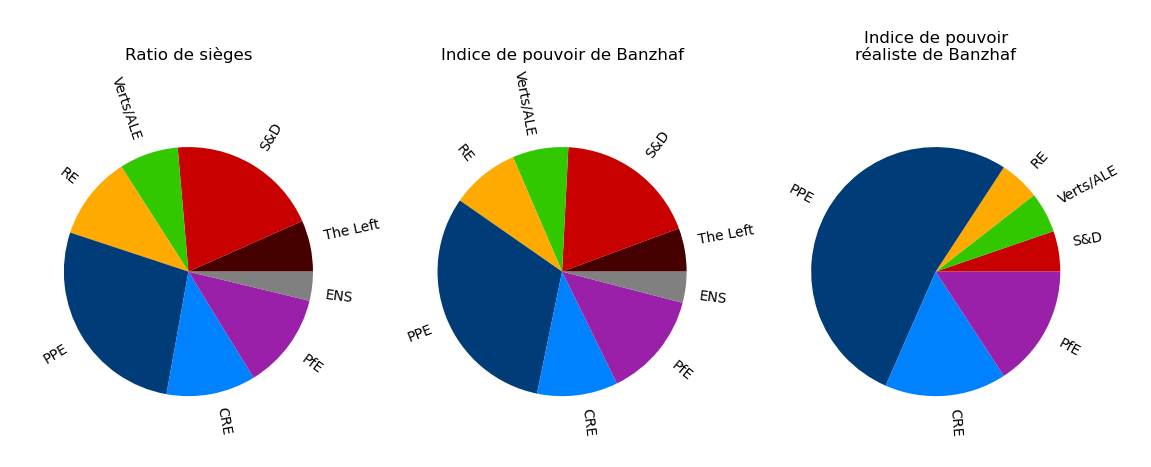
\includegraphics[width=\textwidth]{diagramme_pouvoir_UE_groupe.png}
	\caption{diagramme en camembert représentant les sièges, l'indice de pouvoir de Banzhaf et l'indice de Banzhaf réaliste que détient chaque groupe au Parlement Européen}
\end{figure}

Le parti populaire européen joue un rôle central dans le Parlement Européen simplement grâce au nombre de sièges qu'il détient.

L'indice de Banzhaf réaliste accentue encore la différence de pouvoir entre le PPE et les autres groupe. Ni les groupes à sa gauche (310 membres) ni les groupes à sa droite (192 membres) n'ont la majorité. Les coalitions gagnantes contiennent donc nécessairement le PPE. 
Au contraire, le S\&D, bien que second groupe en terme de nombre de membres, est le deuxième groupe le plus à gauche. Les groupe des Verts/ALE aux ENS peuvent facilement former des coalitions sans le S\&D. Son indice de Banzhaf réaliste est ainsi faible.
De même, les groupes GUE/NGL et ENS situés aux extrémités du Parlement Européen ont un indice de Banzhaf nul puisque toute coalition gagnante réaliste où ils sont, contient aussi le PPE ce qui rend ces deux groupes non décisifs.

\begin{figure}[H]
	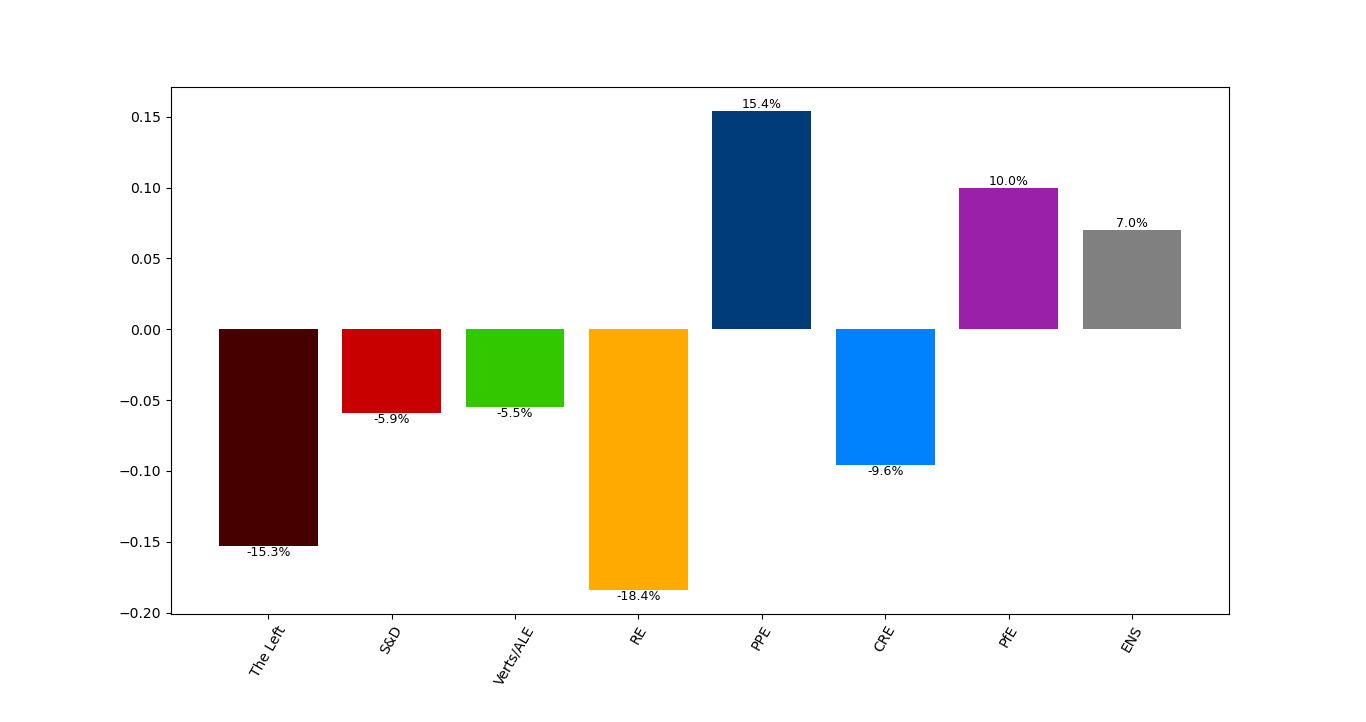
\includegraphics[width=\textwidth]{graph_écart_pourvoir_représentation_groupe.png}
	\caption{diagramme montrant pour chaque groupe l'écart relatif $\nicefrac{(pouvoir - repr\acute{e}sentation)}{repr\acute{e}sentation}$}
\end{figure}

\begin{figure}[H]
	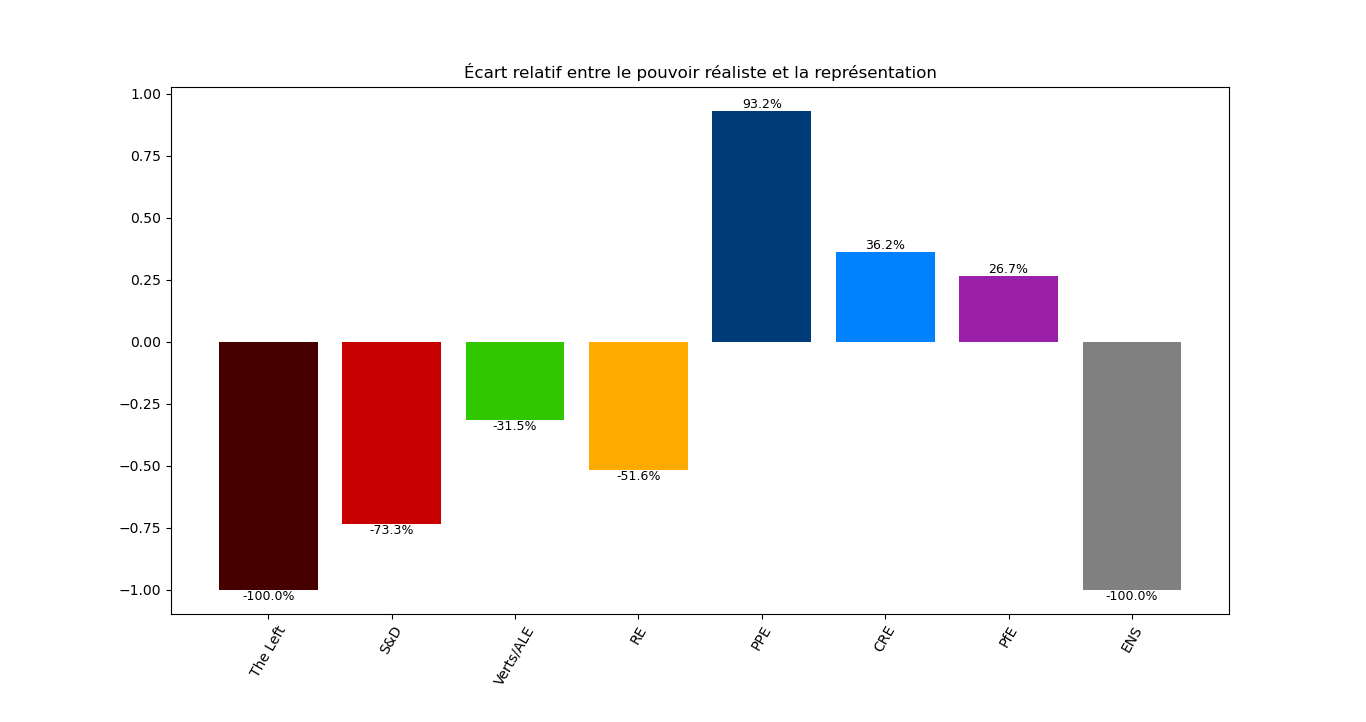
\includegraphics[width=\textwidth]{graph_écart_pourvoir_réaliste_représentation_groupe.png}
	\caption{diagramme montrant pour chaque pays l'écart relatif $\nicefrac{(pouvoir~r\acute{e}aliste - repr\acute{e}sentation)}{repr\acute{e}sentation}$}
\end{figure}
	
	% !TeX root = compte-rendu.tex
% !TeX spellcheck = fr


\section{Le système Penrose 62}
	
	\addcontentsline{toc}{section}{Références}
	\bibliographystyle{plain}
	\bibliography{articles}
\end{document}